\chapter{Методика тестирования}

\section{План приёмочных испытаний приложения}

\subsection{Объект тестирования}

Объектом тестирования является программный модуль для тестирования взаимодействия Flex приложений с сервером через
протокол AMF. Модуль является дополнением к тестовому фреймворку Apache JMeter.

\section{Цели и приоритеты тестирования}

Целью тестирования является проверка соответсвия разработанного программного обеспечения требованиям, установленным
в техническом задании.

\section{Стратегии тестирования}

Функциональное тестирование --- проверка соответствия требованиям, указанным в техническом задании,
применяется к функционалу, за который отвечает разрабатываемый модуль.

\section{Последовательность работ}

\begin{enumerate}
\item Проектирование набора тестовых случаев;
\item Подготовка тестового окружения;
\item Проведение тестирования;
\item Анализ результатов;
\end{enumerate}

\section{Критерии начала тестирования}

\begin{enumerate}
\item законченность разработки требуемого функционала;
\item наличие задокументированных требований к программному обеспечению;
\item наличие набора тестовых случаев;
\item готовность тестового окружения;
\end{enumerate}

\section{Критерии окончания тестирования}

\begin{enumerate}
\item соответствие продукта функциональным требованиям;
\item стабильность работы продукта на протяжении обозначенного периода;
\end{enumerate}

\section{Тестовое окружение}

Для проведения тестирования необходимо следующее программное обеспечение:

\begin{enumerate}
\item сервер BlazeDS;
\item скомпилированное Flex приложение, использующее AMF канал для передачи сообщений;
\item web-браузер c установленным Flash Player;
\item Apache JMeter;
\item Apach Maven;
\end{enumerate}

\section{Сценарии тестирования приложения}

\section{Настройка тестового окружения}

Перед проведением тестов необходимо настроить тестовую среду следующим образом:

\begin{enumerate}
\item установить программное обеспечение, указанное в разделе "Тестовое окружение" плана приёмочных испытаний.
Место установки JMeter далее будем называть JMETER\_HOME;
\item подключить к JMeter тестируемый модуль amf-translator --- добавить jar-файл приложения в каталог
JMETER\_HOME/lib/ext;
\item развернуть Flex приложение на сервере BlazeDS, запустить его и убедиться, что оно функционирует;
\item запустить JMeter --- приложение запускается с помощью файла jmeter.bat или ApacheJMeter.jar, находящихся в
каталоге JMETER\_HOME/bin.
\end{enumerate}

\section{Функциональные тесты}

\subsection{Проверка записи тестовых запросов}

Предусловия:

\begin{enumerate}
\item Добавить элемент AMF Proxy Server (WorkBench > Add > Non-Test Elements > AMF Proxy Server);

\begin{figure}[ht]
\center{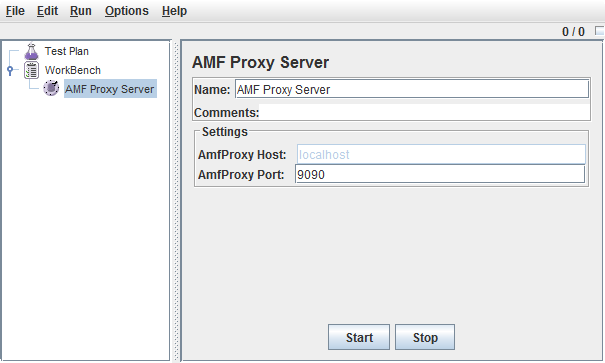
\includegraphics[height=120mm, width=160mm]{fig/development/proxySettings.png}}
\caption{Настройка прокси-сервера}
\label{ris:proxySettings.png}
\end{figure}

\item В поле AmfProxy Port необходимо указать номер порта, который будет слушать наш прокси сервер.
Если указать, например, 9090, то прокси-сервер будет запущен на localhost:9090;
\item Запустить браузер и указать там точно такие же настройки прокси-сервера.
Также стоит убедиться, что указанный Вами порт уже не занят другим приложением;
\item Далее открыть в браузере Flex приложение;
\end{enumerate}

Шаги теста:

\begin{enumerate}
\item Запустить прокси-сервер, нажав кнопку "Start"
\item С помощью браузера ввести данные во Flex приложение и вызвать метод удалённого объект.
\item Завершить запись тестовых запросов, нажав кнопку "Stop"
\end{enumerate}

Ожидаемый результат:

\begin{enumerate}
\item  После завершения записи тестов, в дереве элементов JMeter в качестве дочернего элемента AMF Proxy Server
появился компонент типа AMF RPC Sampler;

\begin{figure}[h]
\center{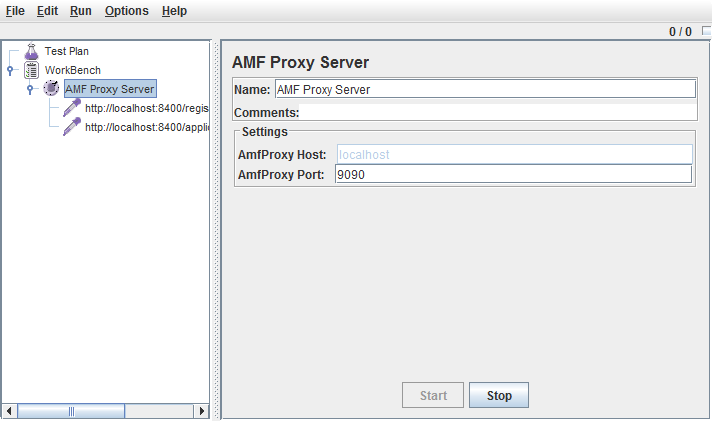
\includegraphics[height=120mm, width=160mm]{fig/development/proxyStart.png}}
\caption{Запуск прокси-сервера}
\label{ris:proxyStart.png}
\end{figure}

\item В AMF RPC Sampler записаны верные параметры AMF запроса, а именно:

\begin{enumerate}
\item Endpoint Url - URL, по которому отправлялся запрос;
\item AMF Call - имя удалённого объекта и процедуы(Например, если мы хоти вызвать у объекта registrationDestionation метод registerUser,
в этом поле следует написать registrationDestination.registerUser);
\item Request Parameters - параметры, переданные методу.
\end{enumerate}

\begin{figure}[ht]
\center{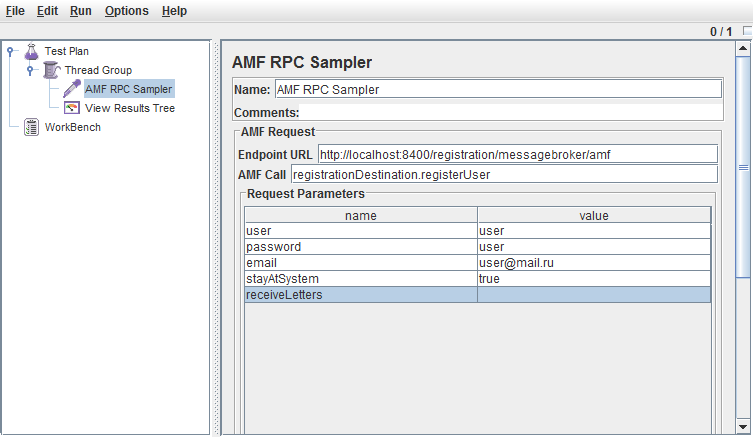
\includegraphics[height=120mm, width=160mm]{fig/development/amfSampler.png}}
\caption{Интерфейс элемента AMF RPC Sampler}
\label{ris:amfSampler.png}
\end{figure}

\end{enumerate}

\subsection{Проверка отправки корректного AMF запроса через AMF RPC Sampler}

Предусловия:

\begin{enumerate}
\item Добавить в Test Plan группу потоков - Thread Group (Test Plan > Threads (Users) > Thread Group).

\begin{figure}[ht]
\center{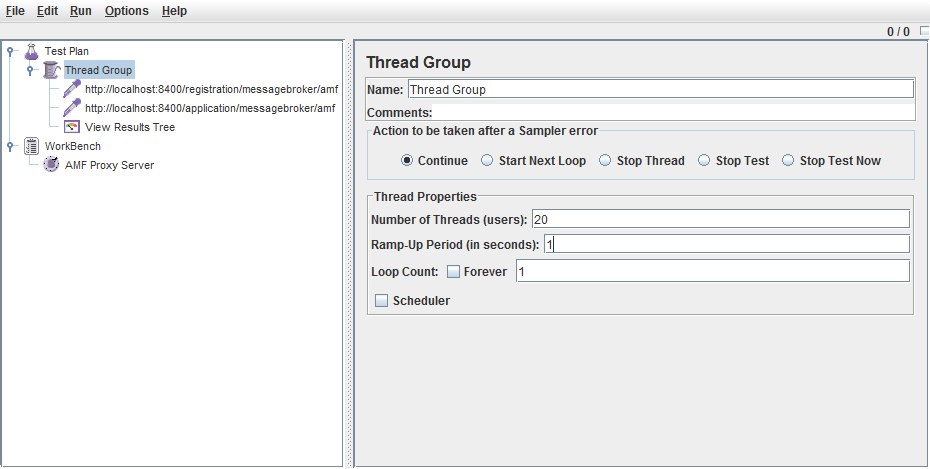
\includegraphics[height=120mm, width=160mm]{fig/development/testplan.png}}
\caption{Создание группы потоков}
\label{ris:testplan.png}
\end{figure}

\item Задать для Thread Group следующие параметры:

\begin{enumerate}
\item Действие, которое будут производиться в случае, если в тест выполняется с ошибкой
(Action to be taken after a Sampler error) --- Continue ;
\item число потоков, в которое будут запускаться шаги тест-плана (Number of Threads) установить равным единице;
\item Интервал, в течение которого будет запущено указанное в предыдущем параметре
число потоков (Ramp-Up Period) установить равным единице;
\item Число повторений набора тестов (Loop Count) установить равным единице;
\end{enumerate}

\item добавить визуалайзер результатов, чтобы иметь возможность отслеживать ход выполнения теста (Thread Group >
Add > Listener > View Results Tree)
\end{enumerate}

Шаги теста:

\begin{enumerate}
\item В Thread Group в качестве дочернего элемента добавить AMF RPC Sampler;
\item Ввести в AMF RPC Sampler все необходимые корректные параметры и запустить содержимое элемента Test Plan (Run > Start);
\item C помощью браузера ввести те же самые данные во Flex приложение и вызвать метод удалённого объекта.
\end{enumerate}

Ожидаемый результат:

\begin{enumerate}
\item После завершения прогона тестов во View Results Tree в дереве элементов тест плана элемент AMF RPC Sampler
посдвечен зелёным цветом (выполнен успешно);
\item на вкладках View Results Tree присутствуют данные запроса и полученного от сервера ответа;
\item Ответ сервера должен быть тем же, что был получен во время вызова процедуры через браузер.
\end{enumerate}

\begin{figure}[ht]
\center{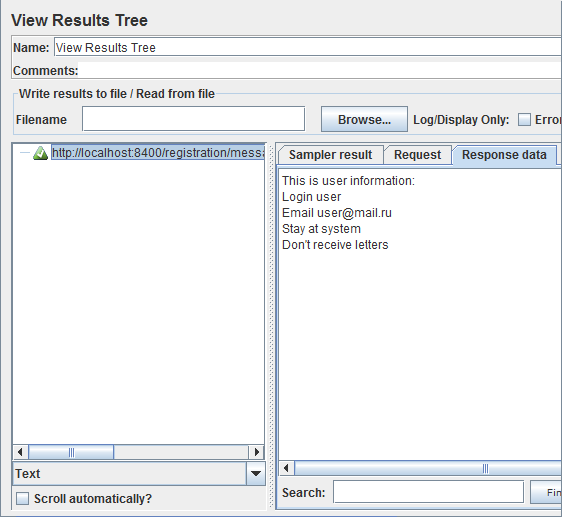
\includegraphics[height=120mm, width=160mm]{fig/development/positiveTest.png}}
\caption{Результаты корректного теста}
\label{ris:positiveTest.png}
\end{figure}

\subsection{Проверка отправки некорректного AMF запроса через AMF RPC Sampler}

Предусловия:

\begin{enumerate}
\item Добавить в Test Plan группу потоков - Thread Group (Test Plan > Threads (Users) > Thread Group).
\item Задать для Thread Group следующие параметры:

\begin{enumerate}
\item Действие, которое будут производиться в случае, если в тест выполняется с ошибкой
(Action to be taken after a Sampler error) --- Continue ;
\item число потоков, в которое будут запускаться шаги тест-плана (Number of Threads) установить равным единице;
\item Интервал, в течение которого будет запущено указанное в предыдущем параметре
число потоков (Ramp-Up Period) установить равным единице;
\item Число повторений набора тестов (Loop Count) установить равным единице;
\end{enumerate}

\item добавить визуалайзер результатов, чтобы иметь возможность отслеживать ход выполнения теста (Thread Group >
Add > Listener > View Results Tree)
\end{enumerate}

Шаги теста:

\begin{enumerate}
\item В Thread Group в качестве дочернего элемента добавить AMF RPC Sampler;
\item Ввести в AMF RPC Sampler неверное имя метода удалённого объекта и запустить содержимое элемента Test Plan (Run > Start);
\end{enumerate}

Ожидаемый результат:

\begin{enumerate}
\item После завершения прогона тестов во View Results Tree в дереве элементов тест плана элемент AMF RPC Sampler
подсвечен красным цветом (тест не пройден);
\item на вкладках View Results Tree присутствуют данные запроса и полученного от сервера ответа;
\item Ответ сервера должен содержать сообщение о соответсвующей ошибке.

\begin{figure}[ht]
\center{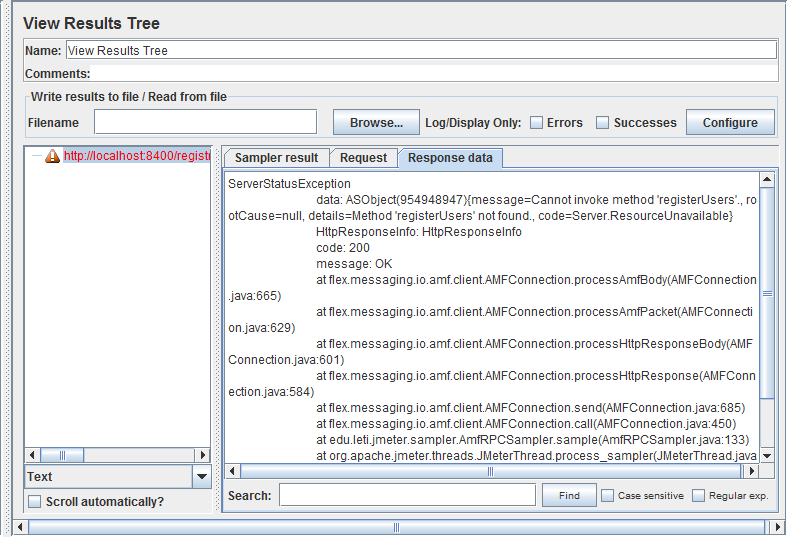
\includegraphics[height=120mm, width=160mm]{fig/development/negativeTest.png}}
\caption{Результаты некорректного теста}
\label{ris:negativeTest.png}
\end{figure}

\end{enumerate}

\subsection{Проверка запуска содержимого Test Plan в несколько потоков}

Предусловия:

\begin{enumerate}
\item Добавить в Test Plan группу потоков - Thread Group (Test Plan > Threads (Users) > Thread Group).
\item Задать для Thread Group следующие параметры:

\begin{enumerate}
\item Действие, которое будут производиться в случае, если в тест выполняется с ошибкой
(Action to be taken after a Sampler error) --- Continue ;
\item число потоков, в которое будут запускаться шаги тест-плана (Number of Threads) установить равным десяти;
\item Интервал, в течение которого будет запущено указанное в предыдущем параметре
число потоков (Ramp-Up Period) установить равным единице;
\item Число повторений набора тестов (Loop Count) установить равным единице;
\end{enumerate}

\item добавить визуалайзер результатов, чтобы иметь возможность отслеживать ход выполнения теста (Thread Group >
Add > Listener > View Results Tree)
\end{enumerate}

Шаги теста:

\begin{enumerate}
\item В Thread Group в качестве дочерних элементов добавить около пяти элементов AMF RPC Sampler;
\item Ввести в элементы AMF RPC Sampler все необходимые корректные параметры и запустить тест план;
\end{enumerate}

Ожидаемый результат:

 После завершения прогона тестов во View Results Tree в дереве элементов все тесты должны быть пройдены ---
 корректный ответ от сервера должен быть получен для каждого элемента.
